\begin{figure}
  \centering
  \begin{subfigure}[b]{0.5\textwidth}
    \centering
    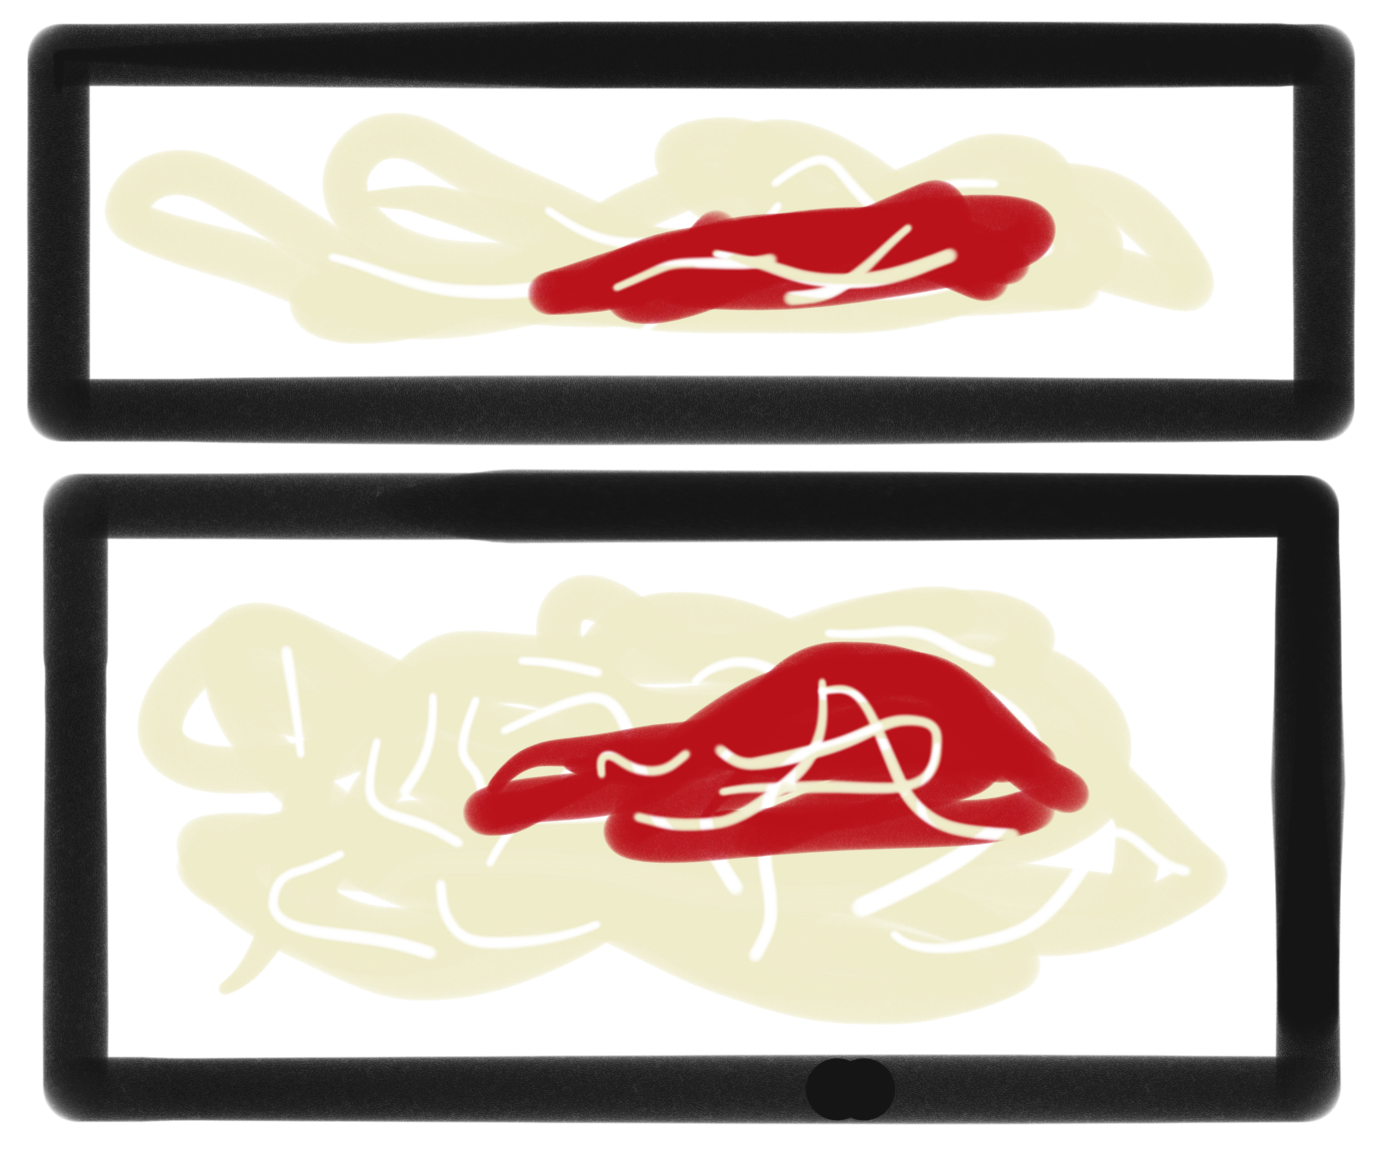
\includegraphics[width=\textwidth]{img/spaghetticode}
    \caption{spaghetti code}
    \label{subfig:spaghetti_code}
  \end{subfigure}%
  \hfill
  \begin{subfigure}[b]{0.5\textwidth}
    \centering
    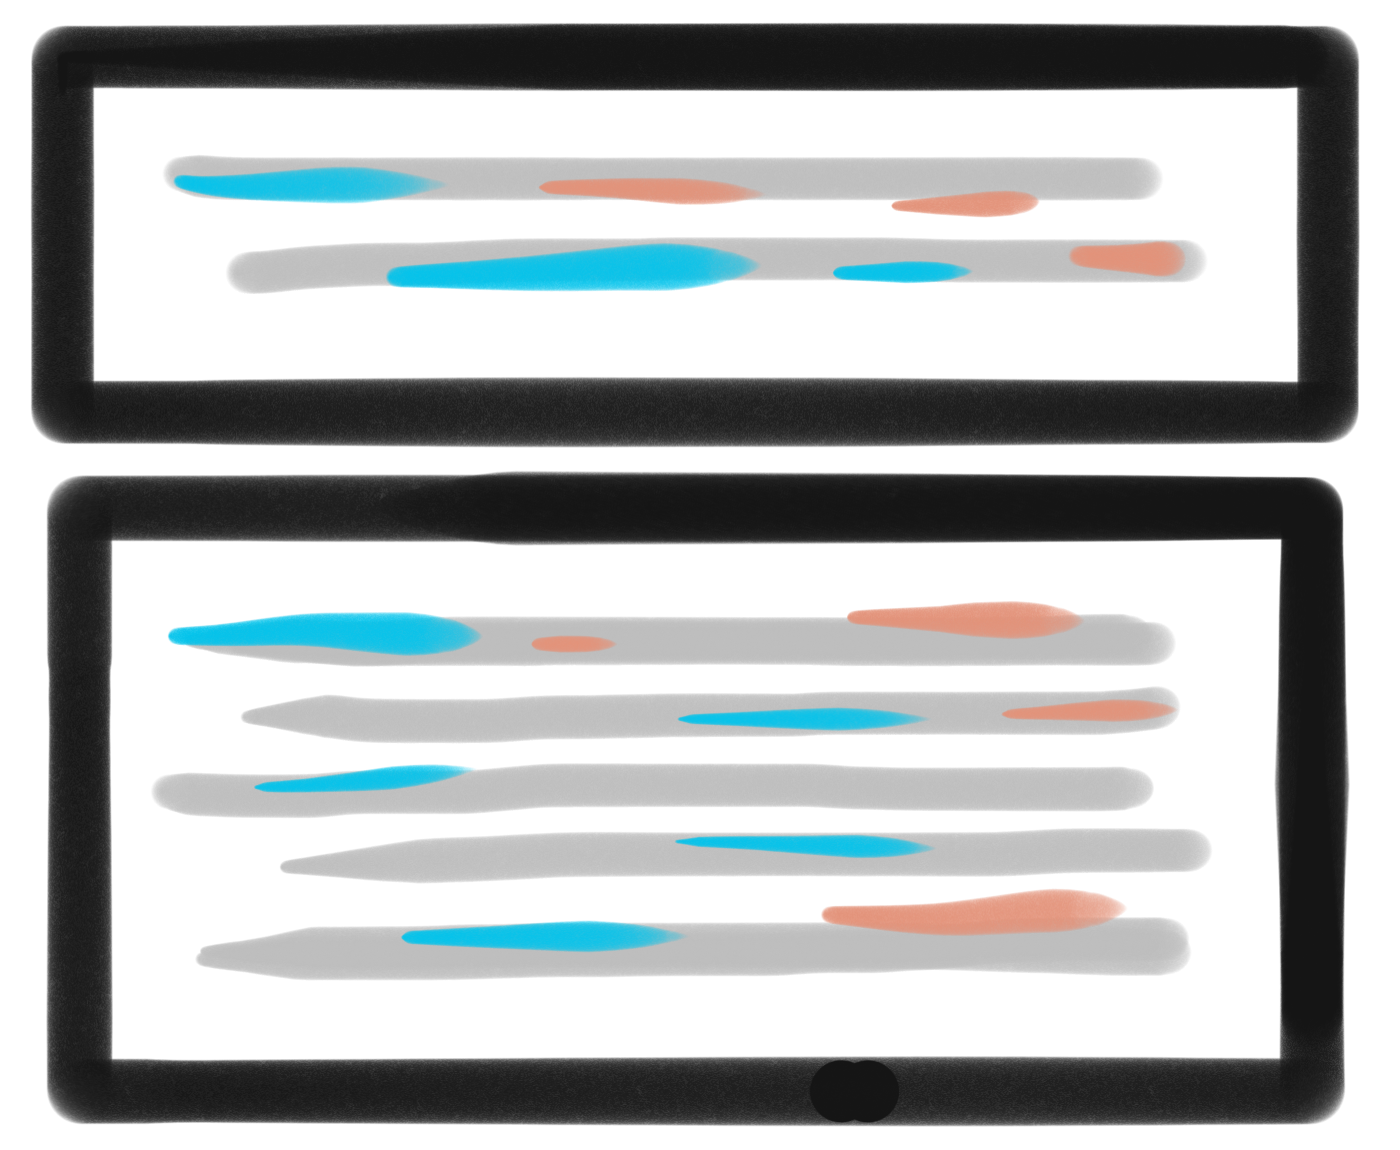
\includegraphics[width=\textwidth]{img/regularcode}
    \caption{regular code}
     \label{subfig:regular_code}
  \end{subfigure}
  \captionsetup{singlelinecheck=off,justification=raggedright}
  \caption{A cartoon comparison of spaghetti and regular code.}
  \label{fig:direct_irregular_vs_indirect_regular}
\end{figure}